\documentclass{article}

\usepackage{ijcai13}
\usepackage{times}
\usepackage{amsmath} 
\usepackage{latexsym} 
\usepackage{ dsfont }
\usepackage{tikz}
\usepackage{graphicx}
\usepackage{subcaption}
\usepackage[ruled,vlined,linesnumbered]{algorithm2e}
\usetikzlibrary{arrows,automata, positioning}

\newtheorem{definition}{Definition}
\DeclareMathOperator*{\argmax}{arg\,max} 

\title{The E-C Algorithm: conceptual bootstrapping via grammar-based
  program compression.}

\author{Eyal Dechter \\
MIT\\
USA \\
edechter@mit.edu
\And
Josh Tenenbaum \\
MIT\\
USA \\
jbt@mit.edu
\And 
Ryan Adams \\
Harvard University\\
USA \\
rpa@seas.harvard.edu}

\begin{document}

\maketitle

\begin{abstract}
Suppose a learner is faced with a set of problems about which it knows
nearly nothing: it doesn't know the distribution of problems, or what
an appropriate loss function might be. For each hypothesized solution
to a problem it gets a few bits of positive or negative reinforcement,
but not enough to steer it effectively in the huge space of possible
solutions. How can such a learner every get off the ground? The key is
to find, by brute force, a solution to one or more simple problems in
that domain and use the information thus gained to pursue subsequent
searches in an informed manner. Here, we formalize this intuition,
where the solution space is the space of typed functional programs and
the gained information is stored as a stochastic grammer over
programs. Specifically, we propose the E-C algorithm, a two step
iterative procedure for exploring such spaces: in the E step, the
learner \emph{explores} a finite subset of the domain for solutions,
guided by a stochastic grammar; in the C step, the learner
\emph{compresses} the successful solutions from the E step to estimate
a new stochastic grammar. As we show in several toy domains, iterating
these two steps quickly propels the learner from a state of solving
almost no problems to solving a large number of problems by gaining
abstract knowledge of the structure of the solution space.
\end{abstract}

\section{Introduction.}

Suppose that, having been shipwrecked and saved by a people with no
knowledge of your language or culture, you find yourself attempting to
communicate in a language about which you know nothing. How would you
go about discovering even the most basic mappings of sounds to
meanings? Overhearing the native speech, you have a sense of what the
phonetics might be like, so you might try various common combinations
of sounds while pointing to things you want. Mostly, you receive
puzzled looks, but if you are lucky, you might pick up on a few key
words or phrases, like ``that'' or ``I want.'' Naturally, you will
proceed to use your discoveries to accelerate your learning, mixing
and matching known phrases to generate new meanings. 

\section{Related work.}

\section{A multi-task program induction problem.}
Our goal is to solve a general multi-task learning problem: we are
given set of \emph{tasks} $T=\{t_k\}_{k=1}^K$ where each task is a
function $t_i : \mathcal{L} \rightarrow \mathds{R} > 0$ which returns
a reward value for every element in the solution representation
language $\mathcal{L}$. Our goal is to find a set of solutions
$X = \{x_k\}_{k=1}^k \subset \mathcal{L}$ such that 

\[
X = \argmax_{x_1, \dots, x_K \in L} \sum_k t_k(x_k).
\]

\section{A compression scheme expresses a belief about the data.}
There is a deep connection between a distribution over data and the
optimally compressive code for that data. In fact, if we know the
probability distribution for a set of observations, we can obtain an
optimally compressive encoding of those observations via arithmetic
coding. Conversely, the encoding generated by a good compression
scheme can be interpreted as an approximation of the data
distribution. 

Take, for example, the Nevill-Manning algorithm for grammar based
compression~\cite{nevill1997identifying}. This algorithm looks for
hierarchical structure in the data and represents that hierarchical
structure as a grammar. The output of the algorithm can be seen as a
grammar and a corresponding parse of the input data. Given that parse,
we can estimate the maximum likelihood probabilistic context-free
grammar for that data~\cite{johnson1998pcfg}. 

\section{The E-C Algorithm.}

In this section, we describe the E-C algorithm and discuss its uses,
applicability, and limitations.

As its name suggests, each iteration of the E-C algorithm consists of
an exploration step and a compression step. In the exploration step,
we enumerate the $N$ most probable hypotheses given our currenst
distribution $D$ over hypotheses. We then assign to each task $t_i$
the hypotheses that match it. We say that a task is \emph{hit} if
there is a least one hypothesis that matches it. In the compression
step, our goal is to assign a single hypothesis $h_i^*$ to each task
$t_i$ such that that resulting set of hypotheses $\{t_i\}$ is as
compressible as possible. The compression this process induces is used
to update distribution $D$.

  \begin{algorithm}
    \SetAlgoLined \KwData{Tasks $T=\{t_1, \dots, t_K\}$,
      distribution $\mathcal{D}_j$ over expressions.}  

    $\text{types} \leftarrow \cup_k \, type(t_k)$. \\
    For $\tau \in \text{ types}$ , $H_N(\tau) \leftarrow$ enumerate
    $N$ most probable elements in $\mathcal{D}_t$ with type $\tau$.\\

    For each \emph{hit} $s_i$ in 
    $T$, $v_{s_i} \leftarrow \{h \in D_j | s_i(h) == True \}$.\\

    $S = \{(s_i, h^*_{s_i})\} \leftarrow$ assignment of elements to tasks s.t. 
    $S$ is most compressible. \\

    $D_{j+1} \leftarrow$ derive new distribution from compression of $S$. \\

    Repeat. 

    \caption{E-C}
  \end{algorithm}



\section{Our implementation.}

\subsection{Representing polymorphically typed programs as binary trees.}

Following~\cite{liang10programs} and~\cite{Briggs:2008}, we use
combinatory logic -- a variable-free subset of the polymorphic
simply-typed lambda calculus lambda calculus~\cite{Pierce_2002} -- as
our program representation language. In short, the combinatory logic
introduces a \emph{basis} of several primitive \emph{combinators} such
that any function in the lambda calculus can be alternatively written
as applications of the basis combinators. Some common basis
combinators are defined as follows:
\begin{align}
I\; x &\rightarrow  x \\
S\; f\; g\; x\; &\rightarrow (f\; x)\; (g\; x) \\ 
B\; f\; g\; x\; &\rightarrow (f\; x)\; g \\ 
C\; f\; g\; x\; &\rightarrow f\; (g\; x) \\ 
\end{align}

The basis combinators can
themselves been expressed in the lambda calculus. The lambda calculus
has two basic operation -- application and abstraction -- but in using
the combinatory logic we sequester uses of the abstraction operation
inside the combinators, and thus have a representation language that
is effectively abstraction- and, thus, variable-free. 

This is very convenient for program synthesis: since every expression
is the application of one expression to another -- with this recursion
bottoming out at the primitive combinators -- each program is a binary
tree. Most importantly, any subtree is itself a well-formed
expression; this is not the case in the lambda calculus, since
abstraction introduces long range dependencies between the $\lambda$
operator and the variables to which that operator refers. In the
lambda calculus, then, a subtree might have free variables, not bound
to any enclosing $\lambda$. 

As a simple example of our representation, consider the squaring
function $\lambda x. * x\; x $. Using two of the basis combinators above,
we can write the squaring function in combinatory logic as $S * I$,
where application associates to the left, so we drop the
parentheses. When we apply this combinator to a value $x$, the action
of the combinator is defined as $S \;*\; I\; x~\rightarrow~(*\; x)\;
(I\; x)~\rightarrow(*\; x)\; x$. Now, we can extend this
representation with a simple polymorphic type
system~\cite{Pierce_2002}. Thus, this combinator can be represented as
a binary tree~(Figure~\ref{fig:clbintree}) whose leaves are typed
primitive combinators and whose interior nodes are typed applications
of combinators.

\begin{figure}
  \centering
  \begin{subfigure}[Before]{0.5\linewidth}
    \begin{tikzpicture}[scale=.7,
        transform shape, level/.style={sibling distance=10mm/#1, font=\scriptsize}
        ]
      \node [font=\scriptsize] (top) {$I$}
      child {node [above=.3cm] (a) {$(I \rightarrow I) \rightarrow I \rightarrow I$}
        child {node [left=.5cm, below=1cm, text width=3cm] 
          {$S : \\(t_2 \rightarrow t_1 \rightarrow t_0)  \rightarrow (t_2 \rightarrow t_1) 
            \rightarrow \\ t_2 \rightarrow t_0$}}
        child {node [right=0cm, text width=2cm] {$*: Int \rightarrow Int \rightarrow Int$}}
      }
      child {node [below right=.3cm and 1cm] (b) {$I \rightarrow I$}
        child {node {$I: t_0 \rightarrow t_0 \rightarrow t_0$}}
      };
    \end{tikzpicture}
    \caption{The typed combinator $S * I$ ($f(x)=x^2$) represented as binary tree.}
    \label{fig:clbintree}
  \end{subfigure}
  \begin{subfigure}[After]{0.4\linewidth}
    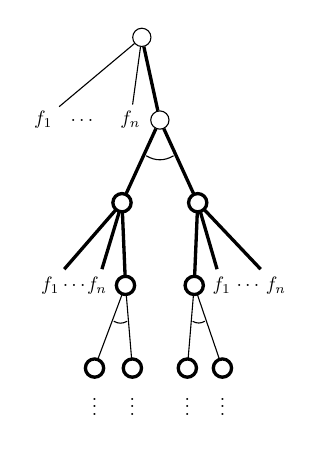
\begin{tikzpicture}[scale=.7, transform shape, 
        level/.style={sibling distance=10mm/#1},
        every edge/.style={draw, thin}
      ]
      \node [circle,draw] (a) {}
      child {node [left=0cm] (b) {$f_1$}}
      child {node [left=.2cm] (c) {\dots} edge from parent[draw=none] }
      child {node [left=.4cm] (e) {$f_n$}}
      child {node [circle,draw, left=1cm] (d) {} edge from parent[very thick]
        child {node [circle, draw, left=.25cm] (l) {} edge from parent[draw=none]
          child {node [left=.5cm] (b) {$f_1$}} 
          child {node [left=.3cm] (c) {\dots} edge from parent[draw=none] }
          child {node [left=.3cm] (e) {$f_n$} edge from parent[very thick]}
          child {node [circle, draw, left=.25cm] (and2) {}
            child {node [circle, draw, left=.25cm](l2) {} edge from parent[draw=none] 
              child {node [above=.5cm] {\vdots} edge from parent[draw=none]}
            }
            child {node [circle, draw] (r2)  {} edge from parent[draw=none] 
              child {node [above=.5cm] {\vdots} edge from parent[draw=none]}
            }
          }
        }
        child {node [circle, draw, right=.25cm] (r) {} edge from parent[draw=none]
          child {node [circle, draw, right=.25cm] (and3) {}
            child {node [circle, draw ](l3) {} edge from parent[draw=none] 
              child {node [above=.5cm] {\vdots} edge from parent[draw=none]}
            }
            child {node [circle, draw, right=.2cm ] (r3)  {} edge from parent[draw=none] 
              child {node [above=.5cm] {\vdots} edge from parent[draw=none]}
            }
          }
          child {node [right=.3cm] (b) {$f_1$} edge from parent[very thick]} 
          child {node [right=.4cm] (c) {\dots} edge from parent[draw=none] }
          child {node [right=.6cm] (e) {$f_n$}}
        }
      };
      
      \path (d)  edge[very thick]  node[inner sep=0mm,pos=.4] (a1) {} node {} (l);
      \path (d)  edge[very thick]  node[inner sep=0mm,pos=.4] (b1) {} node {} (r);
      \path (a1) edge[bend right] (b1) ;

      \path (and2)  edge node[inner sep=0mm,pos=.4] (t0) {} node {} (l2);
      \path (and2)  edge node[inner sep=0mm,pos=.4] (k0) {} node {} (r2);
      \path (t0) edge[bend right] (k0) ;

      \path (and3)  edge node[inner sep=0mm,pos=.4] (t1) {} node {} (l3);
      \path (and3)  edge node[inner sep=0mm,pos=.4] (k1) {} node {} (r3);
      \path (t1) edge[bend right] (k1) ;
    \end{tikzpicture}
    \caption{The space of all typed combinators represented as an
      infinitely deep And-Or tree. Any specific combinator as a
      sub-binary tree of this And-Or tree whose leaves consist of only
      the $f_i$ nodes (i.e., the primitive combinators of the
      grammar).}
    \label{fig:andor}
    \end{subfigure}
  \caption{A typed binary tree representation of the combinator $S\;*\;I\;$.}
\end{figure}

\subsection{Best-first enumeration of most probably programs.}
In order to explore the frontier of most promising programs, we need a
procedure that enumerates the $N$ most probable programs. We can
formulate this naturally as a best-first exploration of an $AND/OR$
tree~\cite{nilsson1982principles}, which we denote $\mathcal{G}$. A
complete program is any binary subtrees of $\mathcal{G}$ whose leaves
coincide with the leaves of $\mathcal{G}$. The tree structure is shown
in Figure~\ref{fig:andor}. The root is an $OR$ node of the requisite
program type. It's children are the primitives of that type $f_1,
\dots, f_n$, and one $AND$ node with two children. Each child of an
$AND$ node has the same structure as the root node, with modified
types: if the type of an $AND$ node is $t$, then the type of its left
child is $\tau \rightarrow t$ (where $\tau$ is a fresh type
variable). Since the type of the right child is constrained by the
subtree rooted at the left child, we always expand the left child
first and use the target type of this left subtree to mark the type of
the right child.

In accordance with the stochastic grammar over programs, we weight all
edges from $OR$ nodes according to the negative log likelihood of
choosing the associated rule from the stochastic grammar, conditioned
on the requesting type. Expanding an $AND$ node has zero cost. In the
case that the stochastic grammar is ill condition, we might have an
infinitely deep solution tree whose cost does not increase as we
unfold it; this can occur, for example, if there are no primitives of
the required type since the log probability of expansion to the next
$AND$ node is 0. . To avoid this, we simply declare a cost for
expanding the next $AND$ node when it is the only node available.

\subsection{Finding the most compressive set of solution.}

Once we have enumerated the best $N$ programs from our distribution,
we will find that some tasks have no solutions and some have one or
more solutions; for those tasks that have solutions, we want to choose
a solution for each task such that the complete set of such solutions
for all the tasks is as compressible as possible.

A natural metric for the compressibility of a set of binary trees is
the number of unique subtrees that this set contains. Thus, we can
attempt to find the assignment of solutions to tasks that minimizes
this value. However, an exact optimization for this problem requires
examining $O(m^k)$ assignments, where $m$ is the maximum number of
solutions for any one task and $k$ is the number of tasks. Since this
is prohibitive, we relax the compressibility metric as follows: we
define the cost of adding each new solution $s_n$ to a partial set of
solutions $s_1, \dots, s_{n-1}$ to be the number of additional unique
subtrees in $s_n$ that are not present in $s_{n-1}$. Our solution thus
becomes approximate and that approximation is order-dependent, but a
depth-first search on the defined search space goes from exponential
in the solution degree to quadratic.

\subsection{Re-estimating the stochastic grammar over programs.}

Given a set of solution programs, we want to re-estimate our
stochastic grammar. Our inspiration for doing this is based broadly on
the Neville-Manning algorithm for grammar-based
compression~\cite{nevill1997identifying}. The idea of that compression
algorithm is to compress any string by creating a grammar for that
string such that a) no two symbols appear more than once in the
grammar and b) every rule is used more than once. From a set of trees
we generate a grammar according to these criteria (though using a less
efficient and much simpler algorithm). 

In our algorithm, we traverse a set of combinator binary trees in
depth first order. We count the occurences of every subtree. Every
time we encounter a subtree for the second time, we designate it as a
primitive in our new grammar. Furthermore, during our traversal, we do
not descend into trees that have been added already to the new
grammar. Thus, we only count an instance of tree if that instance is
not a subtree of a primitive element of the new grammar.

We want to count the number of
times every subtree is encountered when it is not a subtree of a tree
already encountered in our traversal. we simply count the numer of
times each unique subtree appears as the child of a subtree \emph{not
  yet encountered} in the solution set. That is, we traverse the
solution set in depth first order, comparing each tree we encounter to
all the trees we previously encountered; but if we encounter a tree we
have already seen, we do not descend into it. In this traversal, the
set of trees we encounter more than once is the set of terminal nodes
in our new grammar. To estimate the probabilities associated with each
node production, we again traverse the solution set, but these time
for each node where a terminal production takes place we count which
other terminal productions could have taken place. We estimate the
terminal production weight to be the ratio of the number of times that
node was used in the first traversal divided by the number of times it
was used in the second traversal (plus 1, to account for the event of
an $AND$ node expansion). Likewise, we re-estimate the probability of
an $AND$ node expansion by diving the number of such expansions in the
solution set by the number of possible expansions in the solution set.

\section{Experiments.}
\subsection{Symbolic regression.}

In this section, we walk through the performance of our learning
algorithm on a symbolic regression problem. In this problem,
each task is a set of pairs $ (x, f(x))$ where $x \in (0, \dots, 10)$
and $f$ is a polynomial. The goal is to discover a program for each
task that outputs the appropriate value $f(x)$ for each input x. We
assume that the data is noise-free.

The choice of an initial grammar for the algorithm will, of course,
have a big effect on its performance, and so we would like to
characterise this effect. We can divide primitives into roughly two
sets; there are low-level primitives, those that operate on concrete
types like Bool or Double, and these tend to be domain specific. For
example, conrete primitives include $1, 2$, etc., and $f(x) = 3x$. The
other class of primitives are abstract primitives, which can be
characterized by having arguments whose types are primarily function
types, like $(t \rightarrow s), (t \rightarrow s) \rightarrow \text{
  Double },$ etc. Of course, we can construct operators that fall in
between. 

The most abstract operators are those that Liang et. al refer to as
``routers''~\cite{liang10programs}. These operators take the place of
$\lambda$ abstraction in the general lambda calculus: whereas
$\lambda$ abstraction allows us to bind arguments to variables nested
deep inside an expression, without them we need to have operators that
``route'' arguments to the appropriate functions in a nested
expression. 

\begin{definition}[Router~\cite{liang10programs}] A \emph{router} is a combinator
represented by a finite sequence of elements from $\{B, C, S\}$. The
behavior of router $r$ is given by
\[
(r \, f \, g \, x_1 \dots x_{|r|}) = (f \, x_{i_1} \dots x_{i_n}) (g
\, x_{j_1} \dots x_{j_n}),
\]
where $i_1 < \dots < i_n$ are indices $i$ such that $r_i \in \{C, S\}$
and where $j_1 < \dots < j_n$ are indices $j$ such that $r_j \in \{B,
S\}$. Let $\mathcal{R}_k$ be the set of all routers of length equal to
$k$. Let $\mathcal{R}_{\leq k}$ be the set of all routers of length
less than or equal to $k$.
\end{definition}

To analyze the behavior of our algorithm, we will vary the parameters
of the problem along two axes while keeping the learning tasks the
same. Along the first axis, we vary the initial library to which our
learner has access with respect to the its abstractness (i.e., number
of routers) and its concreteness (i.e. number of concrete
primitives). Along the second axis we vary the size of the search
frontier.

Each task is to predict the value of an unknown polynomial on the
inputs $0, \dots, 10$. The set of tasks corresponds to the set of
polynomials $\{ax^2 + bx + c | a, b, c \in \{0, \dots, 10 \}\}$. 

In Figure~\ref{fig:symreg}, we show performance results as we vary
both the routers included and the frontier size. Each individual plot
shows how changing the frontier size changes the number of tasks the
algorithm identifies correctly over the course of ten algorithm
iterations. In addition, we have a baseline for each curve, visits the
same number of expressions as the corresponding algorithm run
(i.e. frontier size $\times$ $\#$ of iterations) but all at once; it
does not do any learning. Thus, this baseline serves as a brute-force
control for the learning aspect of the algorithm. 

\begin{figure}

\includegraphics[width=\linewidth]{figures/learningCurves.pdf}
\includegraphics[width=\linewidth]{figures/performanceFrontierSize.pdf}
\caption{E-C learning curves for the symbolic regression task set as
  we vary the frontier size.}
\label{fig:symreg} 
\end{figure}


Why do the learning curves asymptote early? One might object that a
learning algorithm should continuously improve, if only slowly, as it
is given more time. But in these runs we observe a finite and
permanent performance cap. This is expected: once the learner find a
set of concepts it can explain, if those concepts fill up the
frontier, then there is nothing to spur the learner to incorporate as
yet unsolved tasks. 

To investigate whether this is in fact the case, we can examine the
proportion of expressions in the frontier that match tasks in our task
set; that is, is the learning curve plateauing because the frontier is
heavily redundant, or is it plateuing because the frontier contains
many expressions that do not hit the task set at
all. Figure~\ref{fig:plateau_investigation} shows the proportion of
the expressions in the frontier that hit a task as the frontier sizeincreases.


\subsection{Digital arithmetic}
Having demonstrated the behavior of the E-C algorithm on symbolic
regression, we analyze its performance on tasks involving digital
arithmetic, a class of problems with known modular structure. The
general goal is to discover boolean circuits consisting of a limited
set of gates that perform arithmetic operations on binary number
representations. 


%% The file named.bst is a bibliography style file for BibTeX 0.99c
\bibliographystyle{plain}
\bibliography{ijcai13}
\nocite{*}

\end{document}

